\documentclass[../main.tex]{subfiles}

En las siguiente sección, presentamos una descripción de las tecnologías IPS siguiendo los esquemas presentados (Fig. \ref{fig:tecnologias}), acompañados de fortalezas y debilidades destacables de cada tecnología. \\
Para abordar de forma coherente las tecnologías IPS, procedemos a clasificarlas previamente. Dicha clasificación se puede hacer utilizando varios criterios, uno de los cuales es el tipo de señal utilizada para el posicionamiento. De esta forma, distinguimos señales \textbf{ópticas}, \textbf{acústicas}, \textbf{magnéticas}, de \textbf{radio frecuencia} o \textbf{híbridas}. \\
Además, para cada tecnología abordada en este capítulo, se trataran las diferentes configuraciones que puede tener una misma tecnología (activa, pasiva, etc.), las fortalezas y debilidades destacables y se presentaran una serie de sistemas, de diferente grado de madurez (estudios, patentes, soluciones comerciales, etc.) que se consideran relevantes para los IPS. \\


\begin{figure}[ht]
    \centering
    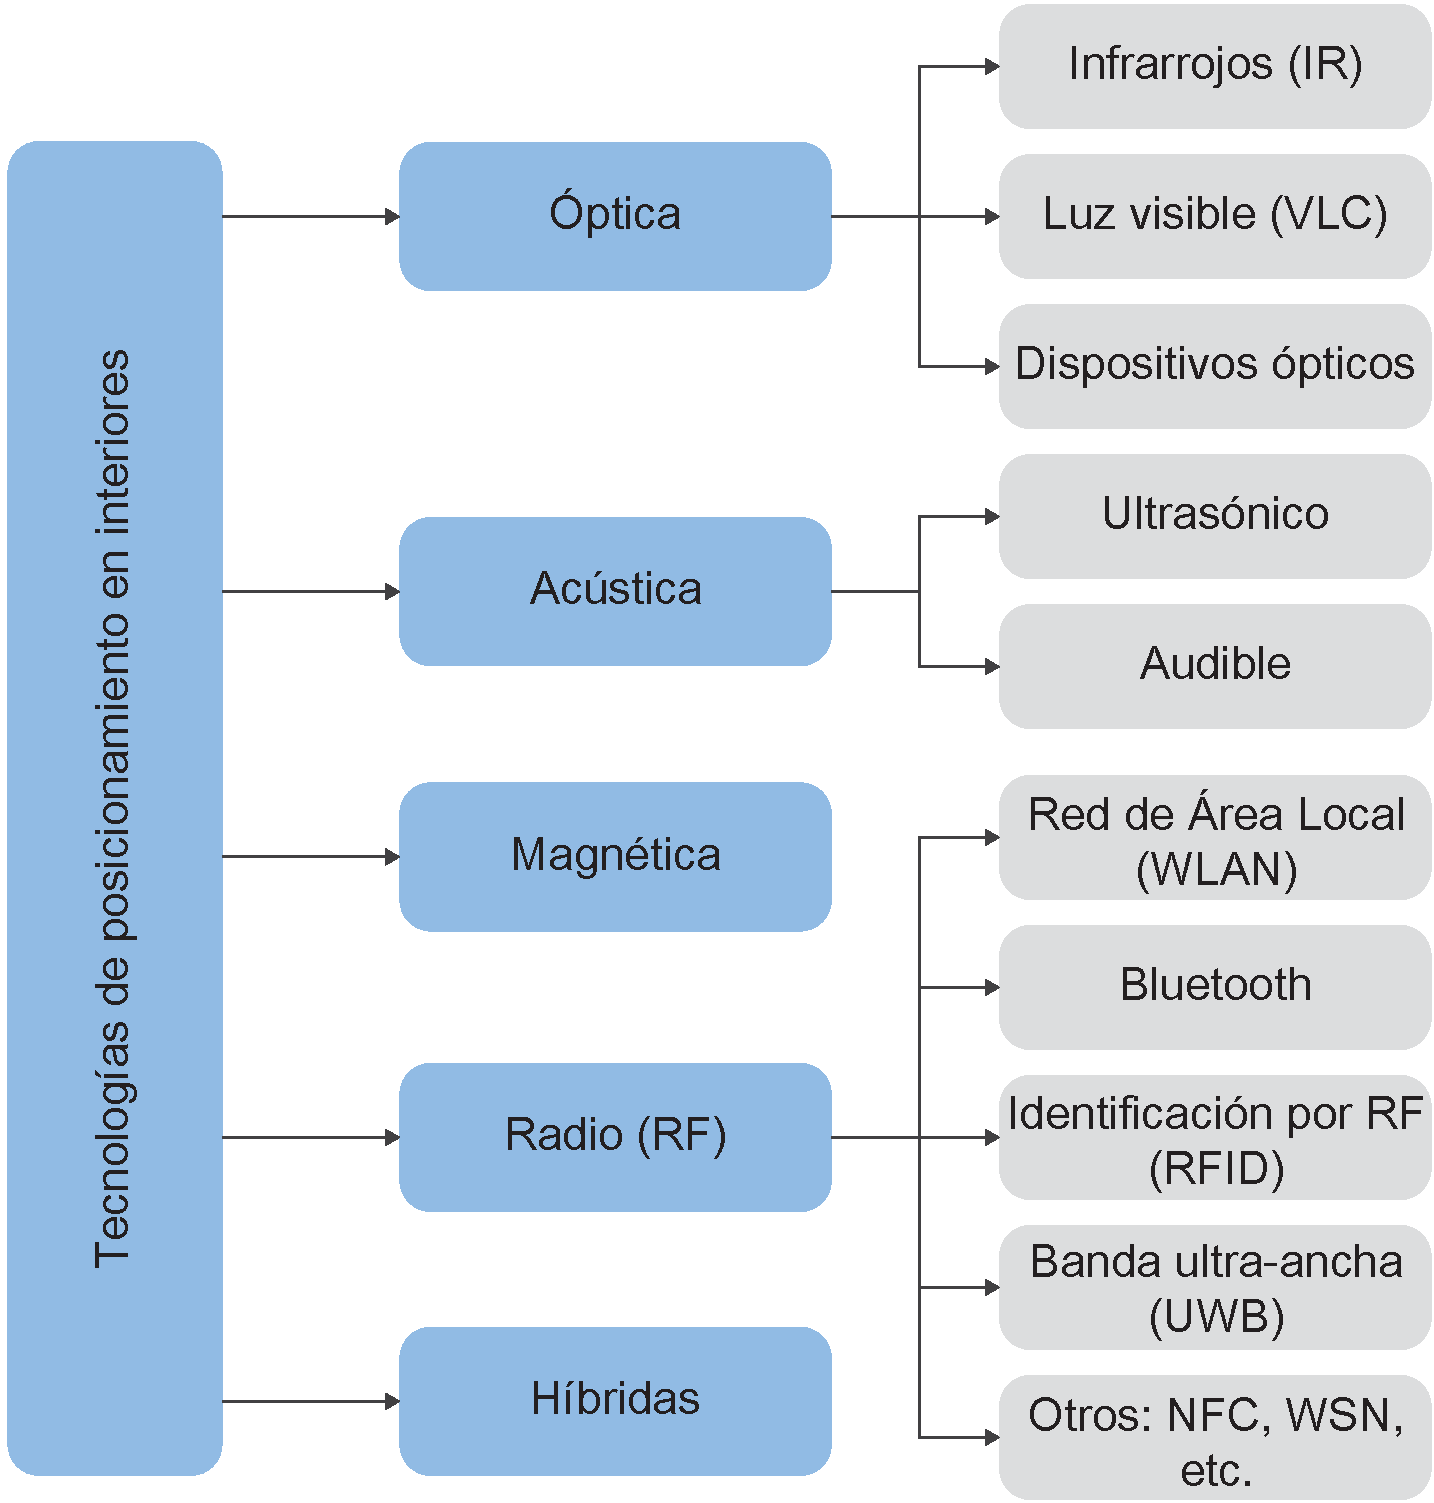
\includegraphics[width=0.7\textwidth]{tecnologias.pdf}
    \caption{Clasificación de tecnologías en IPS.}
    \label{fig:tecnologias}
\end{figure}

\section{Óptica} \label{section:optica}
Aunque las señales ópticas son de hecho solo una forma de radiación electromagnética, se han separado de las ondas de radio, porque las tecnologías específicas son diferentes, así como sus ventajas y desafíos; por ejemplo, las señales ópticas utilizadas en tecnologías de localización están restringidas por línea de visión. \\
Como tecnologías ópticas se distinguen los infrarrojos y la luz visible. Además, se ha aprovechado esta clasificación para tratar en este apartado las tecnologías ópticas no basadas en características radio de la señal sino en dispositivos ópticos, es decir, cámaras y sensores láser.

    \subsection{Infrarroja} \label{subsection:infrarroja}
    La tecnología de infrarrojos (IR) para IPS utiliza radiación electromagnética con longitudes de onda superiores al espectro de luz visible. Un sistema simple de infrarrojos está compuesto por un diodo emisor de luz infrarroja, que emite una señal infrarroja como ráfagas de luz no visible, y un receptor fotodiodo para detectar y capturar los pulsos de luz, que luego se procesan para recuperar la información. El posicionamiento infrarrojo se puede utilizar en configuraciones activas o pasivas. \\
    
    Cabe destacar que uno de los primeros sistemas de posicionamiento en interiores fue un sistema basado en tecnología IR con una configuración activa, \emph{Active Badge} desarrollado por \emph{Want et al.} \cite{want.1992}. Este es un sistema ampliamente utilizado para la ubicación de objetos o personas que lleven una etiqueta, en una red de sensores IR conectados a un servidor centralizado \cite{want.1992}. Existen sistemas más modernos basados en esta tecnología como el propuesto por \emph{Gorostiza et al.} \cite{gorostiza.2011}. \\
    Los sistemas con configuración pasiva prescinden del uso de etiquetas y en su lugar utilizan sensores térmicos para detectar radiación infrarroja por proximidad. Estos sensores no alcanzan los niveles de precisión y rendimiento de la configuración activa. \\
    
    La fiabilidad del sistema IR se ve afectada por muchas características de la señal óptica emitida, como su directividad, así como su forma de reaccionar a los obstáculos, como la reflectividad y la dispersión. La mayoría de los sistemas de IR requieren una línea de visión directa (LoS, \emph{line of sight}) desde el emisor hasta el sensor. Por supuesto, en el contexto de los sistemas IR IPS, el requisito de la eliminación de LoS es una gran desventaja, ya que carece de áreas de no detección que están ocluidas por el transmisor o el sensor, lo que disminuye la usabilidad del sistema. \\
    Para un rango a nivel de sala el coste asociado es muy bajo. Sin embargo, conforme escalamos en la cobertura del sistema, son necesarios mas receptores para mantener la precisión. Como resultado, la complejidad y el coste de la infraestructura se verían aumentados.

    \subsection{Luz visible} \label{subsection:visible}
    La comunicación por luz visible (VLC, \emph{Visible Light Communication}) es una tecnología que utiliza luz visible para transmitir datos. La transmisión de datos mediante luz visible es posible debido a la capacidad de la fuente de luz para encenderse y apagarse en intervalos muy cortos. Este parpadeo puede ser tan rápido que no puede ser percibido por los ojos humanos y puede usar una variedad de métodos de modulación. \\
    Todos los sistemas basados en VLC mantienen una configuración pasiva, debido a que las lámparas son pesadas y tienen un consumo elevado \cite{liu.2010vlc, zhang.2014}. La configuración consiste en que cada una de las lámparas fijas tiene una codificación de parpadeo diferente, por lo que el foto-sensor recibe la luz y compara la modulación con los esquemas de codificación conocidos. Finalmente, determina cuál es el dominante, asociando la ubicación del sensor con la proximidad de la lámpara correspondiente. \\

    Una ventaja de tal disposición es la no intrusividad. Se ha considerado VLC para IPS debido a que permite la reutilización de la infraestructura de luz artificial ya disponible, por lo que el coste de implementación sería bajo para coberturas bajas. Conforme la cobertura aumenta, la complejidad y el coste aumentaría.
    Aunque se puede usar cualquier tipo de lámpara, las luces LED son las más apropiadas. Muchas de las soluciones comerciales (p.e., \emph{Philips} \cite{philips}) usan bombillas dedicadas, lo que aumenta el coste del sistema.

    \subsection{Dispositivos ópticos} \label{subsection:disp_opt}
    Entendemos por dispositivos tecnológicos ópticos a aquellos sistemas ópticos que, valiéndose de cualidades ópticas de la señal, permiten capturan información del entorno. Distinguimos dos dispositivos, cámaras y láser.
    
    \subsection*{Cámara} \label{subsection:camara}
    Existen multitud de cámaras; estáticas, dinámicas, fotográfica, infrarroja, etc. A continuación, se presenta una clasificación según la metodología utilizada en la obtención de la posición \cite{mazuelas.2009}, mencionando brevemente aquellas que resultan más relevantes para este estudio:
    
    \subsubsection{Cámaras de flujo óptico}
    Las cámaras de flujo óptico (\emph{optical flow}) se utilizan para la detección de velocidad, acimut e incremento de posición al comparar un conjunto de imágenes consecutivas. Los rendimientos en precisión están relacionados con el sensor y el algoritmo considerados. Las cámaras de flujo óptico se caracterizan por su tamaño pequeño y peso ligero, con requisitos limitados de capacidades computacionales y un coste aceptable (generalmente dentro de los 100\EURcr{} \cite{li.2018novel}). \\
    Existen algoritmos ampliamente extendidos para extraer la posición gracias mediante \emph{optical flow}, la implementación de estos métodos puede comprobarse el los estudios realizados por \emph{Gageik et al.} \cite{gageik.2013}, por \emph{McGuire et al.} \cite{mcguire.2017}, o por \emph{Moshe et al.} \cite{moshe.2012}.
    
    \subsubsection{Seguimiento de movimiento}
    Los sistemas de seguimiento de movimiento (\emph{motion traking}) consisten en observar un objeto móvil con una o varias cámaras estáticas en tiempo real para determinar la posición del objeto haciendo uso de marcadores reflejados para detectar datos de posición, velocidad y orientación \cite{vicon, optitrack}. \\
    A pesar de sus altos rendimientos, los sistemas de movimiento de la cámara necesitan una infraestructura personalizada y una calibración periódica, que implican un alto coste (30.000\EURcr{} aprox. \cite{li.2018novel}). \\
    Debido a la limitación asociada al coste han surgido versiones de bajo precio y con precisión reducida como los propuestos por \emph{Mustafah et al.} \cite{mustafah.2012}, o por \emph{Tisse et al.} \cite{tisse.2005}.
    
    \begin{figure}[h]
        \centering
        \includegraphics[width=0.6\textwidth]{photos/motion-tracking.PNG}
        \caption{Configuración de los sistemas \emph{motion tracking} \cite{tilch.2010}.}
        \label{fig:conf-motion}
    \end{figure}
    
    \subsubsection{Navegación basado en visión}
    El enfoque de navegación basado en visión (\emph{vision-based navigation}) consiste en una secuencia de imágenes tomadas por una cámara a lo largo de una determinada ruta. En una fase inicial, se captura la ruta, creando una base de datos con las imágenes tomadas en la ejecución. Tras analizar la secuencia de visualización, un usuario puede estimar su propia posición al tomar una imagen de su entorno y comparar haciendo coincidir con las imágenes almacenadas en la secuencia de visualización. \\
    Se conoce como odometría visual (VO, \emph{visual odometry}) el proceso de estimar el movimiento de un agente utilizando solo la entrada de una o varias cámaras conectadas a él \cite{scaramuzza.2011}. La VO tiene muchas variantes: podría involucrar 6 grados de libertad o movimientos más restringidos (como en el caso de un vehículo con ruedas en un piso plano) y podría hacerse con la ayuda de un modelo como un mapa, ya sea disponible previamente (\cite{wang.2010}, \cite{de.2014}) o construida cuando la cámara se está moviendo (también conocida como SLAM, \emph{Simultaneous Location and Mapping} \cite{garcia.2016}, \cite{zhou.2018vslam}).
    
    \subsubsection{Navegación basada en marcadores}
    Los sistemas de posicionamiento óptico que dependen completamente de las características naturales de las imágenes carecen de robustez, en particular en condiciones con iluminación variable. Con el fin de aumentar la robustez y mejorar la precisión de los puntos de referencia, se utilizan marcadores codificados dedicados para sistemas con exigentes requisitos de posicionamiento. \\
    Existen diferentes tipos de marcadores en forma de anillos concéntricos, códigos de barras o patrones que consisten en puntos de colores (ver Fig. \ref{fig:target}). Existen versiones reflectantes y no reflectantes. \\
    
    \begin{figure}[h]
        \centering
        
\includegraphics{photos/target.pdf}
        \caption{Diferentes marcadores usados en la navegación basada en marcadores.}
        \label{fig:target}
    \end{figure}
    
    Los sistemas de navegación basada en marcadores (\emph{marked-based navigation} utilizan marcadores ya que proporcionan tres propósitos para el desarrollo algorítmico: 
    
    \begin{itemize}
        \item Simplificación de la detección automática de puntos correspondientes.
        \item Introducción de la escala del sistema.
        \item Distinción e identificación de objetivos mediante el uso de un código único para cada marcador.
    \end{itemize}
    
    Este tipo de sistemas disponen de dos configuraciones. Si los marcadores se encuentran en el entorno y el objeto a posicionar lleva el dispositivo óptico, el sistema se considera ``pasivo''. En cambio, si el objeto lleva la cámara y en el entorno se encuentran los marcadores el sistema sería ``activo''. \\
    Con el objetivo de ejemplificar este tipo de posicionamiento, se agrega el estudio realizado por \emph{Benini et al.}, un sistema híbrido que utiliza marcadores para parte de su posicionamiento \cite{benini.2013}.
    
    \subsection*{Láser} \label{subsection:laser}
    Los sensores LiDAR (\emph{Light Detection and Ranging}), se pueden clasificar en dos categorías: distanciometro y escáner. El primero se caracteriza por un único rayo láser, proporcionado por el emisor del sensor y reflejado por obstáculos. El tiempo de llegada (ToA) se utiliza para medir una distancia de un solo punto. Los costes del distanciometro varían según el rendimiento considerado, pero se mantienen dentro del rango de 100\EURcr{} a 1000\EURcr{} \cite{li.2018novel}. Por el contrario, los escáneres permiten adquirir información de la nube de puntos gracias a los sistemas de dirección controlada o sistemas de espejo. Los datos de la nube de puntos incluyen la distancia de los obstáculos, según el ToA, los ángulos de orientación, el nivel de reflexión de la superficie y las coordenadas del GPS (solo para los sensores georreferenciados). Además, la gestión de la nube de puntos requiere capacidades computacionales adecuadas. Finalmente, los escáneres son más caros que el distanciometro: el coste varía desde 1,000\EURcr{} hasta 30,000\EURcr{} \cite{li.2018novel}. \emph{Fröhlich y Mettenleiter} proponen en su estudio los principales escáneres en el mercado \cite{frohlich.2004}, entre los que destacan \emph{Velodyne} \cite{velodyne} y \emph{Hokuyo} \cite{hokuyo}. \\
    Entre las soluciones en el mercado se destaca la desarrollada por \emph{Nikon Metrology} \cite{nikon}, conocida como iGPS (\emph{indoor Global Positioning System}) \cite{schmitt.2010igps}. El nombre del sistema es engañoso, pues el funcionamiento del mismo es diferente a su contraparte en exteriores (GPS). \\
    
    El láser infrarrojo o LED son las principales tecnologías utilizadas por los sensores LiDAR. El alto precio de estos sistemas viene justificado por las muy elevadas precisiones conseguidas, normalmente inferior al milímetro \cite{Mautz.2012}. Si bien los láseres permiten un rango de medición largo de un solo punto, hasta 100 m, las dimensiones y el peso hacen que el sensor LiDAR láser no sea adecuado para aplicaciones de UAV ligeras. Los LED infrarrojos, en cambio, suelen ser más ligeros, más pequeños y más baratos que el láser; experimentan menos consumo de energía, sin embargo, sus prestaciones también son limitadas debido a un alcance más reducido del sensor.

\section{Acústica} \label{section:acustica}
Las señales de sonido, que consisten en ondas de presión que se propagan en el aire, se benefician del hecho de que el sonido viaja a una velocidad mucho más lenta que las señales electromagnéticas, lo que permite la medición del tiempo entre la emisión y la llegada de una señal mucho más fácilmente. \\
El tiempo de emisión a menudo se mide transmitiendo simultáneamente una señal de radio y una señal de sonido, ya que la señal de radio llega al sensor casi instantáneamente y la señal de sonido llega al sensor más tarde, por lo que la diferencia entre estos dos tiempos se puede utilizar para calcular la distancia. Por supuesto, también existe la opción de usar ToA o TDoA, también con las ventajas de una señal lenta. \\
Dentro de las tecnologías acústicas, se distinguen los ultrasonidos y las señales audibles:

    \subsection{Ultrasónica} \label{subsection:ultrasonica}
    Los sistemas basados en el posicionamiento ultrasónico utilizan frecuencias de sonido superiores al rango audible (más allá de 20 KHz) para determinar la posición del usuario utilizando el tiempo necesario para que una señal ultrasónica viaje desde un transmisor a un receptor. Una ventaja evidente de las señales de ultrasonido contra señales audibles es que los primeros no son detectables por los humanos, mientras que los últimos serían molestos. 
    Muchos son los sistemas IPS consolidados que utilizan esta tecnología entre los que destacan \emph{Active Bat} \cite{ward.1997}, \emph{Cricket} \cite{priyantha.2000} y \emph{DOLPHIN} \cite{fukuju.2003, minami.2004}. \\
    Los sistemas de ultrasonido, como muchos otros IPS, pueden ser ``activos'' o ``pasivos''. Sistemas como \emph{Active Bat} poseen una configuración activa, en el que se utiliza una serie de micrófonos fijos en el entorno y una etiqueta que lleva el objeto.
    En cambio, la configuración pasiva consiste en una serie de transmisores (etiquetas) en el entorno y un receptor (micrófono) llevado por el objeto. Esta estructura es la utilizada por los sistemas \emph{Cricket} y \emph{DOLPHIN}. \\
    En ambos casos, la ubicación del usuario se calcula principalmente mediante multilateración, se necesitan al menos 3 micrófonos o balizas para encontrar la posición del objeto. \emph{Cricket} utiliza también métodos por proximidad para estimar la localización.  \\
    Un sistema comercial actual utilizado en robótica es \emph{Marvelmind} \cite{marvelmind} que obtiene una gran precisión mediante una configuración pasiva y multilateración. \\
    En general, los sistemas pasivos consiguen mejores resultados en relación a la escalabilidad y la precisión debido a que al aumentar el número de etiquetas se producen colisiones entre las señales transmitidas. \\

    \begin{figure}[h]
        \begin{subfigure}{0.5\textwidth}
            \includegraphics[height=6cm, width=0.9\linewidth]{photos/dolphin.PNG}
            \caption{Balizas DOLPHIN \cite{fukuju.2003, minami.2004}.}
            \label{fig:dolphin}
        \end{subfigure}
        \begin{subfigure}{0.5\textwidth}
            \includegraphics[height=6cm, width=0.9\linewidth]{photos/ultrasounds.jpg}
            \caption{Balizas Marvelmind \cite{marvelmind}.}
            \label{fig:marvelmind}
        \end{subfigure}
         
        \caption{Balizas utilizadas en sistemas de ultrasonidos.}
        \label{fig:ultrasonidos}
    \end{figure}

    \subsection{Audible} \label{subsection:audible}
    También es posible utilizar señales de sonido audibles para codificar información para sistemas de localización. Por supuesto, la ingenua idea de solo emitir un sonido audible artificial tiene demasiados inconvenientes, principalmente que molestaría a los humanos cercanos. Pero existen esquemas más sofisticados, como la marca de agua sobre un sonido ya disponible, como la música en centros comerciales y otros lugares públicos de una manera no detectable para el oído humano. \\
    La totalidad de estos sistemas utilizan configuración pasiva y la posición es obtenida mediante multilateración. Beep \cite{mandal.2005}, BeepBeep \cite{peng.2012} o GuoGuo \cite{liu.2013guoguo} son un ejemplo de sistemas que utilizan esta tecnología.

\section{Magnética} \label{section:magnetica}
Si bien existen algunos enfoques para la localización en interiores utilizando campos magnéticos generados artificialmente, la mayoría de los sistemas modernos utilizan la fuerza y/o la orientación del campo magnético natural de la Tierra para realizar el posicionamiento. Debido a esto, durante este trabajo solo vamos a considerar los sistemas basados en los recursos naturales de la Tierra y su campo magnético. \\
Los IPS magnéticos utilizan magnetómetros para medir las variaciones del campo magnético, que se utilizará para determinar la posición del objeto. La estimación de la posición se realiza comúnmente a través de métodos tales como \emph{fingerprinting} \cite{haverinen.2009} aunque también existen sistemas que usan técnicas de multilateración con campos magnéticos artificiales, los cuales no abordaremos en este estudio. \\
Aunque pueda parecer una técnica actual, el posicionamiento mediante campos magnéticos es una práctica que se lleva realizando desde hace años \cite{raab.1979}. Existen sistemas comerciales que utilizan esta tecnología, como \emph{IndoorAtlas} \cite{indooratlas} que utiliza \emph{fingerprinting} magnético junto con otras tecnologías para extraer la localización. \\
Aunque estos sistemas carezcan de una estructura costosa y no sufran por errores por línea de visión directa, tienen otras desventajas. Los sistemas se ven limitados en su cobertura, la cual aumentar supone incrementar en gran medida la complejidad y el coste del sistema. Además, el \emph{fingerprinting} magnético se ve afectado por las estructuras metálicas de los edificios que reduce la precisión obtenida.

\section{Radio frecuencia} \label{section:rf}
Las tecnologías de radio frecuencia (RF) son aquellas que utilizan señales RF para determinar la posición del objeto.
El término RF, que está relacionado con la frecuencia de las señales de radio, tiene los beneficios de que su señal puede penetrar paredes y obstáculos que conducen a un área de cobertura más amplia, así como también reutiliza las infraestructuras de RF existentes, lo que resulta en una reducción de costes. \\
Estos sistemas hacen uso de las técnicas de multilateración, \emph{fingerprinting} y de detección por proximidad. En esta sección se abordan:

\begin{itemize}
    \item Red inalámbrica de área local (WLAN).
    \item Bluetooth.
    \item Identificación por radio-frecuencia (RFID).
    \item Banda ultra-ancha (UWB).
    \item Comunicación por campo cercano (NFC).
    \item Red de sensores inalámbricos (WSN).
\end{itemize}

Las diversas tecnologías de posicionamiento RF tienen fortalezas y limitaciones únicas, que las siguientes subsecciones resaltan.

    \subsection{Red inalámbrica de área local} \label{subsection:wlan}
    La red inalámbrica de área local (WLAN, \emph{Wireless Local Area Network}), también conocida como Wi-Fi, es una tecnología para la transmisión y recepción de datos mediante ondas electromagnéticas, lo que proporciona conectividad inalámbrica dentro de un área de cobertura. Fue definido por el estándar IEEE 802.11 como sustituto al par trenzado, la fibra coaxial o fibra óptica utilizada para transmitir datos en una LAN convencional. \\
    Mientras que para el posicionamiento en el exterior es suficiente para obtener la identificación de una estación base detectable (es decir, el nombre simbólico o SSID de un punto de acceso), en la ubicación en el interior es necesario ir más allá de la mera identificación del punto de acceso para lograr una mejor precisión. Normalmente se utilizan dos enfoques para localizar a un objeto que utiliza la tecnología WLAN:
    
    \begin{itemize}
        \item Multilateración: mediante el RSSI de varias bases Wi-Fi conocidas se puede resolver la posición \cite{mazuelas.2009}.
        \item \emph{Fingerprinting}: un patrón de bases de Wi-Fi conocidas con sus RSSI se compara con una base de datos de patrones conocidos asociados con ubicaciones \cite{bahl.2000, yim.2008}. Otra opción, es usar el modelo de propagación de una o varias antenas conocidas, calculando la distancia a la base conocida. \\ Por supuesto, esto requiere una actividad de mapeo previa extensa y almacenar patrones de Wi-Fi para cada punto mapeado para construir la base de datos.
    \end{itemize}
    
    Una de las primeras propuestas con esta tecnología fue la desarrollada por \emph{Bahl et al.} , conocida como RADAR \cite{bahl.2000}. Esta propuesta utiliza el \emph{fingerprinting} junto con los patrones de RSSI y la ayuda del algoritmo \emph{k-NN}. Existen otros muchos sistemas inspirados en este con variaciones del algoritmo, de los patrones registrados, etc., pero con resultados similares \cite{yim.2008}. \\
    Existen también soluciones que utilizan multilateración para determinar la posición \cite{mazuelas.2009}. Sin embargo, debido a la precisión obtenida mediante RSSI, son más comunes los sistemas híbridos que utilizan una combinación de ambos enfoques \cite{hongpeng.2007}.
    
    \subsection{Bluetooth} \label{subsection:bluetooth}
    Bluetooth es una tecnología de comunicación inalámbrica que utiliza información incorporada digitalmente en las señales de radiofrecuencia. Originalmente pensado para el intercambio de datos en distancias cortas, fue definido por el estándar IEEE 802.15.1. Los principales objetivos de la tecnología son facilitar la comunicación entre dispositivos móviles y fijos o dos móviles, para eliminar cables y conectores entre dispositivos y para facilitar la sincronización de datos entre dispositivos personales. \\
    La tecnología Bluetooth se ha considerado para los sistemas de posicionamiento en interiores como un competidor de Wi-Fi, en particular desde la adopción generalizada de Bluetooth Low Energy (BLE) \cite{gomez.2012}, debido a su disponibilidad, de bajo coste y muy bajo consumo de energía, lo que permite que los emisores fijos funcionen con baterías durante varios meses o incluso años. \\
    Los sistemas de posicionamiento basados en Bluetooth también son llamados \emph{Bluetooh Local Positioning Application} (BLPA) \cite{kotanen.2003}. Al igual que la tecnología anterior, existen dos enfoques para posicionar un objeto. Por un lado, la ubicación se puede estimar mediante multilateración y RSSI. Por otro lado, mediante \emph{fingerprinting} puedo extraer la posición \cite{kotanen.2003, hallberg.2003}. \\
    Entre las soluciones comerciales encontradas destaca \emph{Apple's iBeacon} \cite{ibeacon}, una propuesta muy madura en el mercado, basada en BLE \cite{gomez.2012}.
    
    \subsection{Identificación por radio-frecuencia} \label{subsection:rfid}
    La identificación por radiofrecuencia (RFID) es una tecnología que utiliza ondas de radio para hacer que un circuito especializado produzca una respuesta que contenga un identificador único. Un sistema RFID consta de lectores RFID y etiquetas RFID. Las etiquetas se pueden clasificar según la forma en que obtienen energía para responder a un lector RFID: pueden ser ``pasivas'' si responden a un lector utilizando solo la pequeña energía emitida por el lector, recolectada por medio de una pequeña antena, o ``activas'' si tienen su propia fuente de alimentación y transmiten periódicamente su señal de identificación. Algunas etiquetas RFID son ``semipasivas'', utilizan una pequeña batería y transmiten solo cuando se detecta una señal del lector. \\
    
    \begin{figure}[h]
        \centering
        \includegraphics[width=0.8\textwidth]{photos/rfid.png}
        \caption{Esquema de funcionamiento de un sistema RFID pasivo \cite{uchitomi.2010rfid}.}
        \label{fig:rfid}
    \end{figure}
    
    Los sistemas RFID se han utilizado para el posicionamiento, especialmente cuando la ubicación del usuario no se necesita saber todo el tiempo, solo cuando se pasa por importantes lugares de control. En estos casos, la ubicación del objeto a menudo se da en forma de una ubicación lógica, como, por ejemplo, en el arco, dentro de la sala, etc., y no en un sistema de coordenadas. \\
    Son posibles dos variantes de posicionamiento del objeto: en una de ellas, el objeto lleva la etiqueta, y la etiqueta es leída por los lectores en la infraestructura. La otra opción es que el usuario lleve un lector, y muchas etiquetas están incrustadas en lugares clave de un área determinada. La primera opción ha sido la más popular por una buena razón: las etiquetas son baratas y muy ligeras, mientras que los lectores son voluminosos y muy caros. \\
    Algunos sistemas populares de localización RFID son Spot ON \cite{hightower.2000spoton} y LANDMARC \cite{ni.2003landmarc}. LANDMARC calcula la posición mediante detección por proximidad (RSSI) y \emph{fingerprinting} haciendo uso del algoritmo \emph{k-NN}. En cambio, Spot ON obtiene la posición mediante multilateración RSSI.
    
    \subsection{Banda ultra-ancha} \label{subsection:uwb}
    La tecnología de banda ultra-ancha (UWB, \emph{Ultra-wide band}) se basa en la transmisión de formas de ondas electromagnéticas formadas por una secuencia de pulsos muy cortos que utilizan un ancho de banda muy grande (ver Fig. \ref{fig:uwb}).
    
    \begin{figure}[h]
        \centering
        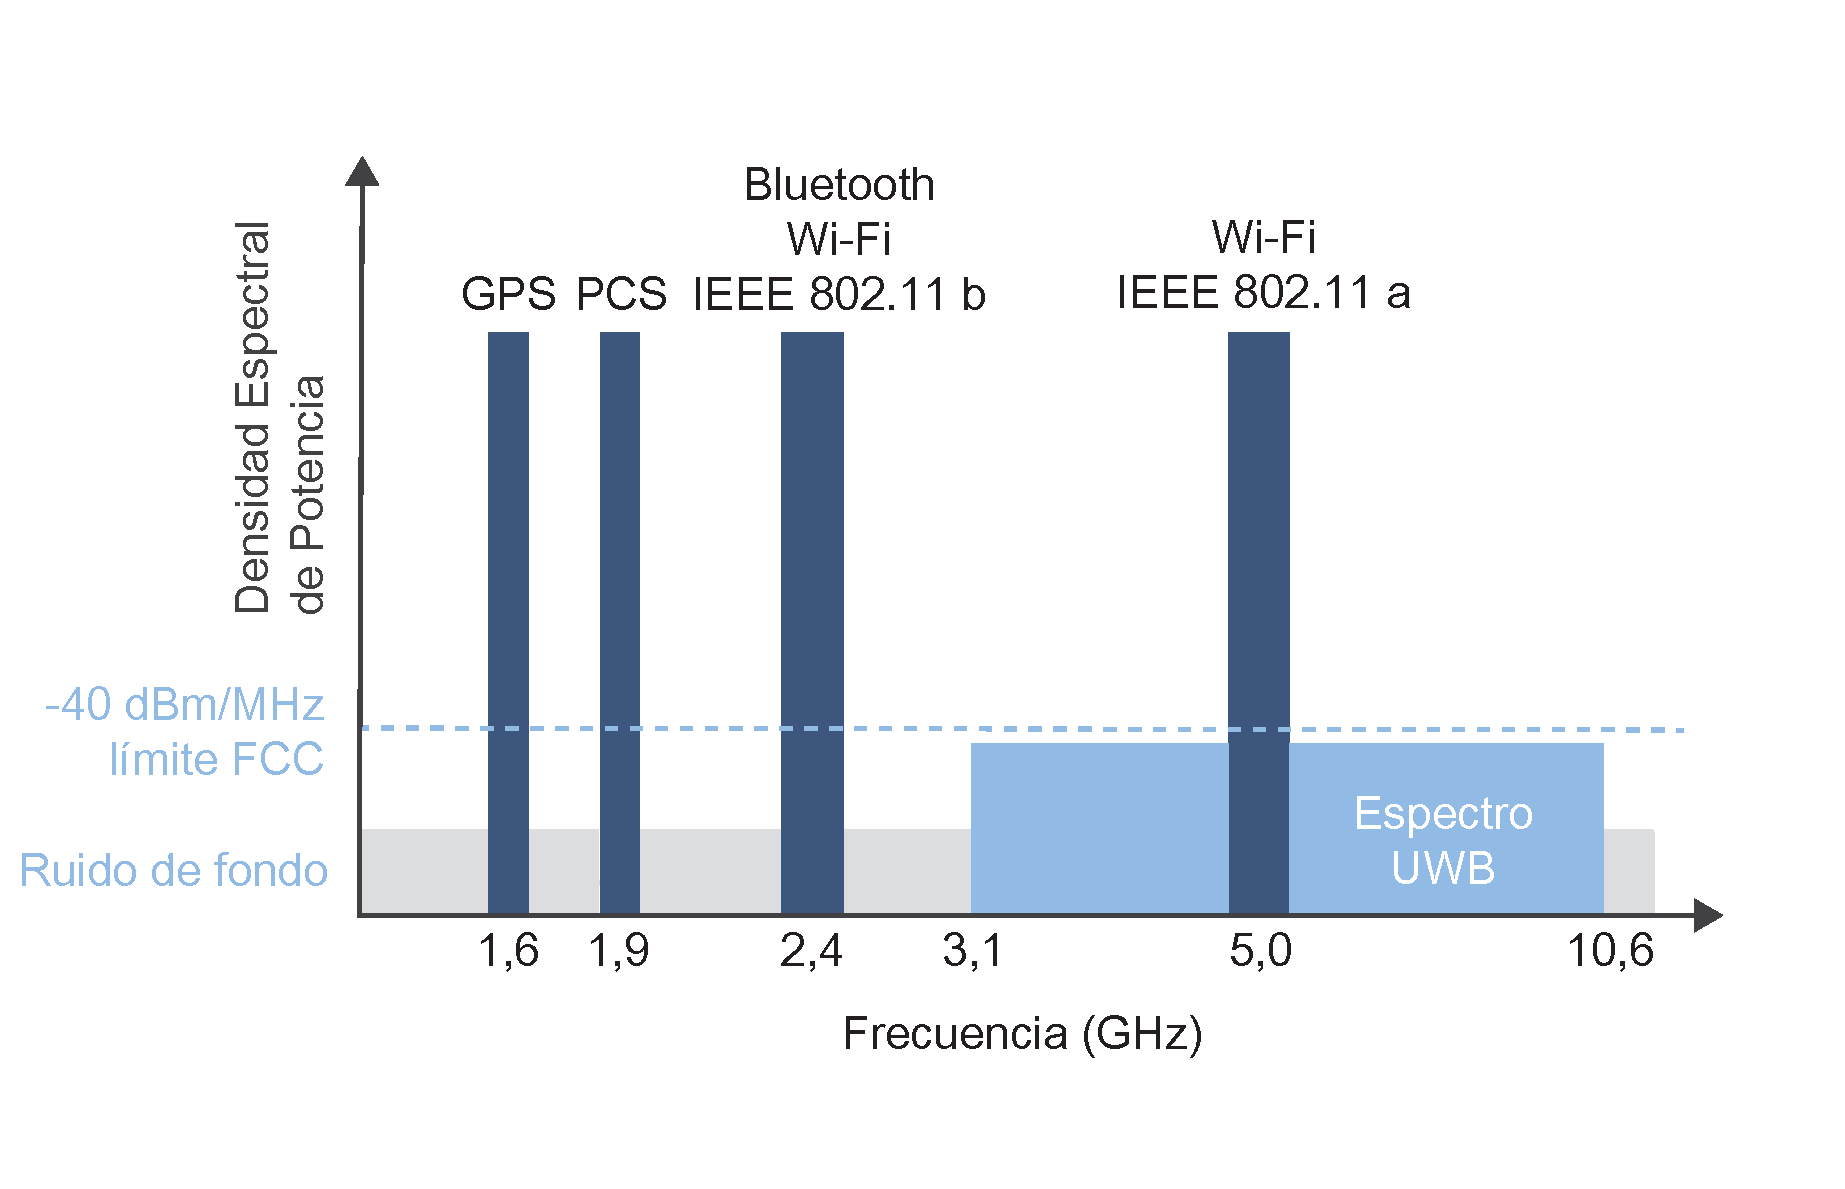
\includegraphics[width=0.9\textwidth]{photos/uwb.pdf}
        \caption{Espectro regulado de UWB \cite{Mautz.2012}.}
        \label{fig:uwb}
    \end{figure}
    
    Se ha considerado la tecnología UWB para los sistemas de posicionamiento en interiores porque las técnicas UWB ofrecen distintas ventajas en la precisión de la medición del tiempo de vuelo, la no necesidad de linea de visión directa (LoS), la inmunidad de múltiples rutas y los requisitos de baja potencia para una operación prolongada. En la gran mayora de sistemas, el posicionamiento se realiza mediante multilateración con ToA, TDoA y/o AoA, aunque también existen sistemas que realizan el posicionamiento mediante \emph{fingerprinting}. \\
    Un ejemplo de un sistema comercial basado en UWB es Ubisense Real-Time Location System (RTLS) \cite{steggles.2005ubisense, ubisense}, el cual utiliza TDoA y AoA mediante multilateración para posicionar la posición. Otras alternativas serían BeSpoon \cite{bespoon}, Decawave \cite{decawave, campbell.2015decawave} y ATLAS \cite{tiemann.2016atlas, tiemann.2018atlas}. Las dos primeras proponen otras soluciones comerciales, mientras que la última, ATLAS, propone una solución de código abierto.
    
     \subsection{Comunicación por campo cercano} \label{subsection:nfc}
     La tecnología de posicionamiento por comunicación por campo cercano (NFC, \emph{Near Field Communication}) es como un sistema de posicionamiento basado en RFID. La diferencia radica principalmente en la distancia de comunicación, el uso de dispositivos móviles por NFC y el cálculo de la posición en un servidor por el sistema RFID. La principal desventaja con el sistema de posicionamiento NFC es que no hay una actualización automática de la posición del usuario. En otras palabras, no hay posicionamiento en tiempo real durante la navegación. \\
     El sistema de posicionamiento NFC consta de tres componentes principales, una etiqueta pasiva, un lector y una base de datos. Mientras que el lector, que es un dispositivo móvil NFC, lee el contenido de la etiqueta pasiva, la base de datos es una ubicación centralizada donde se almacenan los datos del mapa interior de un edificio. El sistema de posicionamiento NFC es un área novedosa en IPS que está ganando terreno gradualmente. \\
     El sistema de posicionamiento NFC involucra un dispositivo móvil NFC que toca a las diversas etiquetas NFC distribuidas dentro de un edificio para determinar la posición actual. En el punto donde el usuario toca una etiqueta, la ubicación de la etiqueta se toma como la ubicación del usuario en ese momento. Esta es una manera simple, efectiva y precisa de determinar una ubicación. Además, la reducción de costes, así como la mejora de la velocidad, la precisión y la eficacia, son los objetivos del desarrollo de un sistema de posicionamiento. \\
    
    \subsection{Red de sensores inalámbricos} \label{subsection:wsn}
    Otra tecnología empleada en los sistemas de posicionamiento de RF es la red de sensores inalámbricos (WSN, \emph{Wireless Sensor Network}). Una WSN está compuesta por un grupo de sensores colaborativos con infraestructuras de comunicación para el monitoreo y registro de condiciones físicas o ambientales, como temperatura, sonido, presión, humedad, luz y viento, para la organización y transmisión de datos a una ubicación central o servidor a través de una WLAN. Una WSN consta de pocos o varios nodos de sensores que son pequeños, livianos y portátiles. El coste del sensor es variable y depende de su consumo de energía, velocidad computacional, ancho de banda y memoria. \\
    El sistema WSN determina y rastrea la posición de una persona o un objeto utilizando señales de las mediciones tomadas por nodos de sensores conectados en red en posiciones conocidas en un edificio. Los sistemas de posicionamiento basados en WSN se pueden implementar de tres maneras, basados en distancia (multilateración), basados en proximidad y basados en \emph{fingerprinting}. \\
    En general, los sistemas basados en distancia tienen una mayor precisión de posición. Sin embargo, estos sistemas tiene una configuración compleja, lo que resulta en un alto coste. Por lo tanto, un despliegue a gran escala no es práctico. \\
    En general, los algoritmos de posicionamiento que utilizan WSN determinan la posición de los nodos del sensor utilizando el conocimiento de las posiciones absolutas de unos pocos sensores y mediciones entre sensores. Además, los sistemas de posicionamiento basados en WSN son difíciles de implementar debido a las limitaciones experimentadas con el sensor con respecto al rango de comunicación, la potencia de procesamiento, la eficiencia energética, la capacidad de respuesta, la robustez, la autoconfiguración y los recursos informáticos. \\
    
    ZigBee, un protocolo estándar de comunicación inalámbrica IEEE 802.15.4, es un dispositivo de radio implementado como un sensor en una WSN, conectado en red a través de una WLAN \cite{wheeler.2007}. \\
    Además, ZigBee se ha utilizado para desarrollar sistemas de posicionamiento en interiores \cite{wheeler.2007} porque es una tecnología de bajo coste y bajo consumo de energía y porque es fácil obtener niveles RSSI ya que estos se incorporan en cada uno de los paquetes enviados, sin necesidad de hardware adicional. \\
    Un sistema de posicionamiento en interiores basado en ZigBee está compuesto por una red de sensores y algoritmos de red de sensores inalámbricos. La mayoría de los algoritmos utilizados en estos sistemas utilizan los valores de RSSI junto con las características de propagación para estimar la ubicación. Por ejemplo, \emph{Larranaga et al.} utilizan ZigBee junto a \emph{fingerprinting} para obtener el posicionamiento \cite{larranaga.2010}. \emph{Alhmiedat y Yang} obtienen la localización mediante proximidad \cite{alhmiedat2008zigbee}. Y \emph{Fang et al.} proponen un sistema híbrido en el que predomina la ubicación mediante multilateración \cite{fang.2012}.

\section{Híbridas} \label{section:hibrida}
Los sistemas que se basan en la fusión de tecnologías se denominan ``híbridos''. En otros estudios, el término ``híbrido'' se refiere a la combinación de diferentes técnicas como AoA, TDoA, etc. En este documento, ``híbrido'' se refiere a la combinación de diferentes tecnologías y/o técnicas indistintamente. En un sistema híbrido, una de las tecnologías suele considerarse más relevante para estimar la ubicación del usuario, mientras que el resto de las tecnologías se consideran complementarias y se utilizan para mejorar las características del sistema, como la precisión y el área de cobertura. \\

Para concluir el capítulo, se presenta la Tabla \ref{table:tecn-algorit} con las tecnologías tratadas, los métodos de posicionamiento asociados y las diferentes alternativas comentadas durante esta sección. La comparativa de tecnologías se hará en la siguiente sección, pues su análisis es más complejo y es necesario introducir ciertos conceptos previos para una correcta descripción de los mismos. \\

    \begin{table}[h]
    \centering
    \begin{threeparttable}
        \begin{tabular}{l c c c}
            \toprule
            \multicolumn{2}{c}{\thead{Tecnología}} & \thead{Algoritmo} & \thead{Referencia} \\
            
            \midrule
            \multirow{7}{*}{Óptica} & \multirow{2}{*}{Infrarrojos} & Multilateración & Active Badge \cite{want.1992}, \cite{gorostiza.2011} \\
                                    &                              & Proximidad      & IR Pasivo \\
                                    \cline{2-4}
                                    & \multirow{2}{*}{VCL}         & Multilateración  & Philips \cite{philips}, \cite{liu.2010vlc, zhang.2014} \\
                                    &                              & Proximidad  & \cite{liu.2010vlc, zhang.2014} \\
                                    \cline{2-4}
                                    & \multirow{6}{*}{Dispositivos} & \multirow{2}{*}{Multilateración} & \emph{Motion tracking} \cite{vicon, optitrack}, \cite{mustafah.2012, tisse.2005} \\
                                    &                               &                                  & LiDAR \cite{schmitt.2010igps, nikon} \\
                                    &                               & Proximidad                       & \emph{Marked-based} \cite{benini.2013} \\
                                    &                               & \multirow{3}{*}{Fingerprinting}  & \emph{Optical Flow} \cite{gageik.2013, mcguire.2017, moshe.2012}, \\
                                    &                               &                                  &  \emph{Vision-based} \cite{wang.2010, de.2014, garcia.2016, zhou.2018vslam}, \\
                                    &                               &                                  &  \emph{Marked-based} \cite{benini.2013} \\
            \midrule
            \multirow{3}{*}{Acústica} & Audible                       & Multilateración & Beep \cite{mandal.2005}, BeepBeep \cite{peng.2012}, GuoGuo \cite{liu.2013guoguo} \\
                                      \cline{2-4}
                                      & \multirow{3}{*}{Ultrasonidos} & \multirow{2}{*}{Multilateración} & Active Bat \cite{ward.1997}, Cricket \cite{priyantha.2000}, \\
                                      &                               &                                  & DOLPHIN \cite{fukuju.2003, minami.2004}, Marvelmind \cite{marvelmind} \\
                                      &                               & Proximidad & Cricket \cite{priyantha.2000} \\
            \midrule
            \multicolumn{2}{c}{\multirow{2}{*}{Magnética}} & Multilateración & Campos artificiales \\
            \multicolumn{2}{c}{}                           & Fingerprinting & IndoorAtlas \cite{indooratlas}, \cite{haverinen.2009} \\
            \midrule
                                & \multirow{2}{*}{WLAN} & Multilateración & RADAR \cite{bahl.2000} \\ 
                                &                       & Fingerprinting  & RADAR \cite{bahl.2000} \\ 
                                \cline{2-4}
                                & \multirow{2}{*}{Bluetooth} & Multilateración & iBeacon \cite{ibeacon} \\ 
                                &                            & Fingerprinting & iBeacon \cite{ibeacon} \\
                                \cline{2-4}
                                & \multirow{3}{*}{RFID}  & Multilateración & Spot ON \cite{hightower.2000spoton} \\ 
            Radio               &                        & Proximidad & LANDMARC \cite{ni.2003landmarc} \\ 
            Frecuencia          &                        & Fingerprinting & LANDMARC \cite{ni.2003landmarc} \\
                                \cline{2-4}
                                & \multirow{3}{*}{UWB} & \multirow{2}{*}{Multilateración} & Ubisense \cite{ubisense, steggles.2005ubisense}, BeSpoon \cite{bespoon}, \\ 
                                &                      &                                  & Decawave \cite{decawave, campbell.2015decawave}, ATLAS \cite{tiemann.2016atlas, tiemann.2018atlas} \\ 
                                &                      & Fingerprinting                   & - \\
                                \cline{2-4}
                                & NFC  & Proximidad & - \\
                                \cline{2-4}
                                & \multirow{3}{*}{WSN}  & Multilateración & ZigBee \cite{fang.2012} \\ 
                                &                       & Proximidad & ZigBee \cite{alhmiedat2008zigbee} \\ 
                                &                       & Fingerprinting & ZigBee \cite{larranaga.2010} \\ 
            \bottomrule
            \addlinespace[1ex]
        \end{tabular}
        
    \end{threeparttable}
    
    \caption{Resumen de las tecnologías de posicionamiento en interiores.}
    \label{table:tecn-algorit}
    \end{table}
